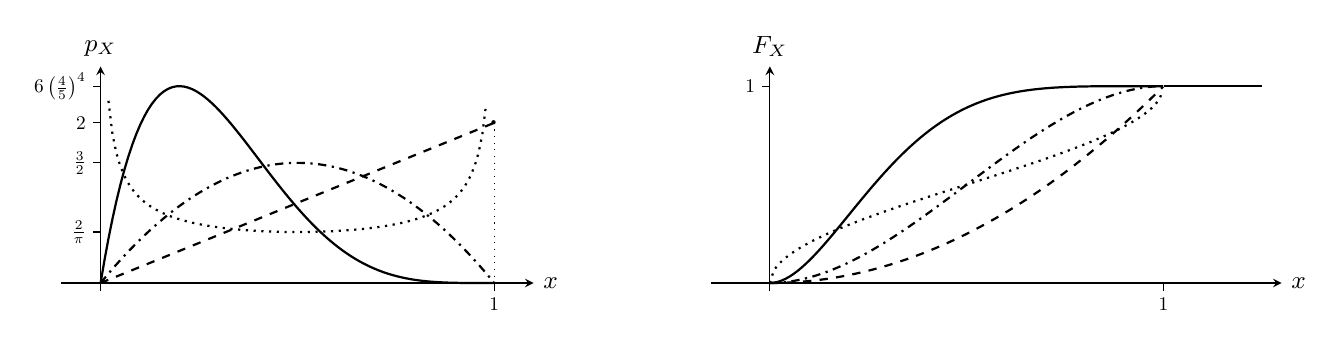
\begin{tikzpicture}%[scale=.9]
\shorthandoff{>}
%
\pgfmathsetmacro{\sx}{5};% x-scaling
\pgfmathsetmacro{\b}{5};% tercera eleccion de (2,beta)
\pgfmathsetmacro{\r}{.05};% radius arc non continuity F_X
%
%
% densidad
\begin{scope}
%
\pgfmathsetmacro{\sy}{2.5*((\b/(\b-1))^(\b-1))/(\b+1)};% y-scaling 
\draw[>=stealth,->] (-.5,0)--({\sx+.5},0) node[right]{\small $x$};
\draw[>=stealth,->] (0,-.1)--(0,2.75) node[above]{\small $p_X$};
%
%\draw[thick] (-.25,0)--(0,0);\draw (\r,\r) arc (90:270:\r);
%\draw[thick] (\sx,0)--({\sx+.25},0);\draw ({\sx-\r},{-\r}) arc (-90:90:\r);
% (a,b) = ( .5 , .5 )
\draw[thick,dotted,domain=.02:.98,samples=100] plot ({\x*\sx},{\sy*1/(pi*sqrt(\x*(1-\x)))});
% (a,b) = ( 2 , 1 )
\draw[thick,dashed,domain=0:1,samples=100] plot ({\x*\sx},{\sy*2*\x}) node[scale=.4]{$\bullet$};
\draw[dotted] (\sx,{2*\sy})--(\sx,0);
% (a,b) = ( 2 , 2 )
\draw[thick,dash dot,domain=0:1,samples=100] plot ({\x*\sx},{\sy*6*\x*(1-\x)});
% (a,b) = ( 2 , b_3 )
\draw[thick,domain=0:1,samples=100] plot ({\x*\sx},{\sy*\b*(\b+1)*\x*((1-\x)^(\b-1))});
%}
%
\draw (0,{\sy*2/pi})--(-.1,{\sy*2/pi}) node[left,scale=.7]{$\frac2\pi$};
\draw (0,{\sy*2})--(-.1,{\sy*2}) node[left,scale=.7]{$2$};
\draw (0,{\sy*1.5})--(-.1,{\sy*1.5}) node[left,scale=.7]{$\frac32$};
\draw (0,{\sy*(\b+1)*((1-1/\b)^(\b-1))})--(-.1,{\sy*(\b+1)*((1-1/\b)^(\b-1))}) node[left,scale=.7]{$6 \left(\frac{4}{5} \right)^4$};
\draw (\sx,0)--(\sx,-.1) node[below,scale=.7]{$1$};
%
\end{scope}
%
%
% reparticion
\begin{scope}[xshift=8.5cm]
%
\pgfmathsetmacro{\sy}{2.5};% y-scaling 
%
\draw[>=stealth,->] (-.75,0)--({\sx*1.25+.25},0) node[right]{\small $x$};
\draw[>=stealth,->] (0,-.1)--(0,{\sy+.25}) node[above]{\small $F_X$};
%
% cumulativa
\draw[thick] (-.5,0)--(0,0); \draw[thick] (\sx,\sy)--({\sx*1.25},\sy);
% (a,b) = ( .5 , .5 )
\draw[thick,dotted,domain=0:1,samples=100] plot ({\x*\sx},{\sy*(.5+asin(2*\x-1)/180)});
% (a,b) = ( 2 , 1 )
\draw[thick,dashed,domain=0:1,samples=100] plot ({\x*\sx},{\sy*(1-(1+\x)*(1-\x))});
% (a,b) = ( 2 , 2 )
\draw[thick,dash dot,domain=0:1,samples=100] plot ({\x*\sx},{\sy*(1-(1+2*\x)*((1-\x)^2))});
% (a,b) = ( 2 , b_3 )
\draw[thick,domain=0:1,samples=100] plot ({\x*\sx},{\sy*(1-(1+\b*\x)*((1-\x)^\b))});
%
\draw (0,\sy)--(-.1,\sy) node[left,scale=.7]{$1$};
\draw (\sx,0)--(\sx,-.1) node[below,scale=.7]{$1$};
\end{scope}
%
\end{tikzpicture}